% \section*{Appendix \hypertarget{AppA}{A}} \label{sec:AppendixA}
\section*{Appendix A} \label{sec:AppendixA}
% \section*{Appendix \hypertarget{AppA}{A}}
% \label{sec:AppendixA}

 
For the sake of completeness and documentation, the usual time- and spanwise-averaged statistics are shown for the b1.4 simulation. They are compared with those of the ZPG case to analyse the APG effects for a wide range of Reynolds numbers. The lower-$\Rey$ APG simulations b1 and b2 are used to compare the effects of different APG intensities at low Reynolds numbers.


% -------- Retau & Retheta --------------------------------
\begin{figure}
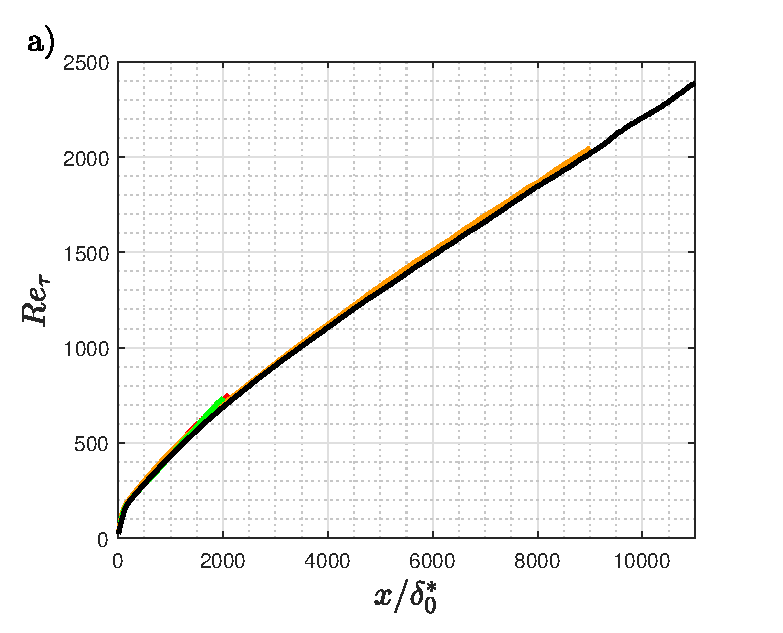
\includegraphics[width=0.49\textwidth]{fig19a.eps}
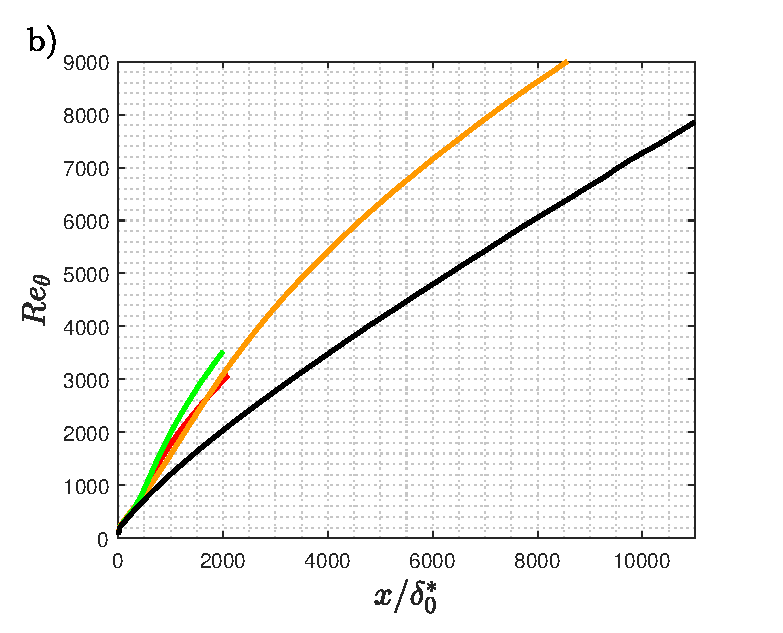
\includegraphics[width=0.49\textwidth]{fig19b.eps}
  \caption{Streamwise development of the a) friction Reynolds number $Re_{\tau}$ and b) Reynolds number based on momentum thickness $Re_{\theta}$ as a function of the streamwise coordinate $x/\delta^{*}_{0}$.  Colors: (\protect\blackline) ZPG; (\protect\orangeline) b1.4; (\protect\redline) b1; (\protect\greenline) b2.}
%   Colors as in table \ref{tab:param}.}
\label{fig:RetauRetheta}
\end{figure}


In figure \ref{fig:RetauRetheta} we show the development of the Reynolds number based on friction velocity ($\Rey_{\tau}=u_{\tau}\delta_{99}/\nu$) and momentum thickness ($\Rey_{\theta}=U_{e} \theta / \nu$) along the streamwise coordinate $x/\delta_0^*$.
The evolution of $\Rey_{\tau}$, which corresponds to the development of the boundary-layer thickness in viscous units $\delta_{99}^+$, is very similar for all the simulations. 
The effects of the APG are more noticeable in the evolution of $\Rey_{\theta}$ where the APGs starts to diverge from the ZPG around $x/\delta_0^*\approx 200$ ($\Rey_{\theta}\approx 400$) and among the APGs the divergence is seen at $x/\delta_0^*\approx 400$ ($\Rey_{\theta}\approx 700$). 

%   --------Cf & H12----------------------------------------
 \begin{figure}
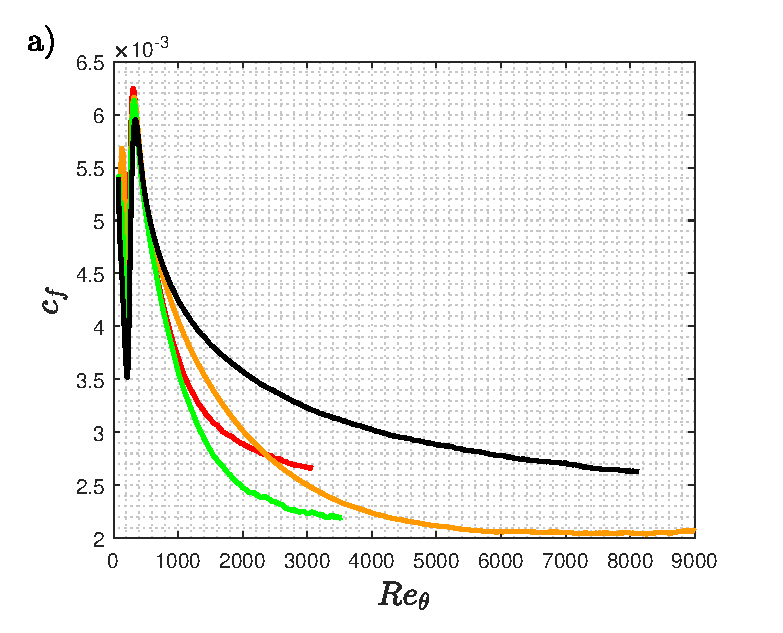
\includegraphics[width=0.49\textwidth]{fig20a.eps}
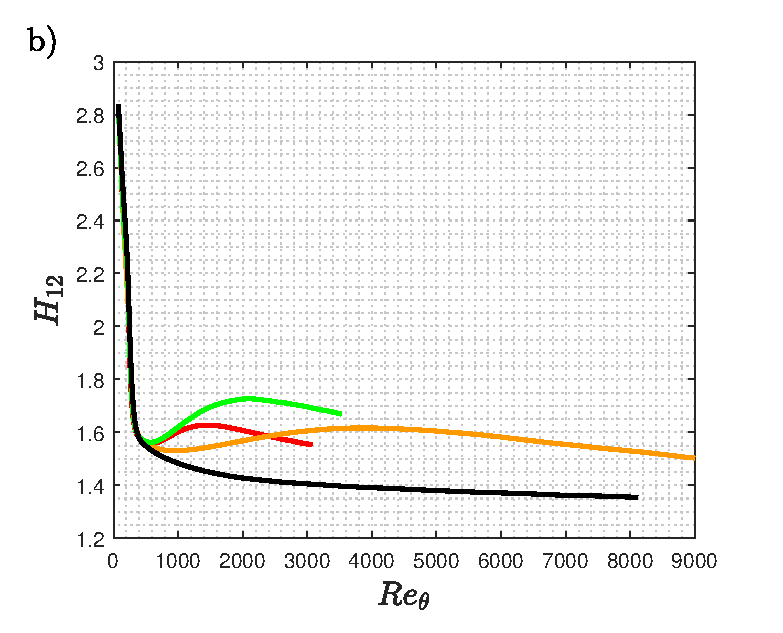
\includegraphics[width=0.49\textwidth]{fig20b.eps}
  \caption{Evolution of a) the skin-friction coefficient $c_f$ and b) the shape factor $H_{12}$ as a function of the momentum-thickness-based Reynolds number $Re_{\theta}$.  Colors: (\protect\blackline) ZPG; (\protect\orangeline) b1.4; (\protect\redline) b1; (\protect\greenline) b2.}
%   Colors as in table \ref{tab:param}.}
\label{fig:cfH12}
\end{figure}
In figure \ref{fig:cfH12} we show the skin-friction coefficient $c_f=2(u_\tau/U_{e})^2$ and the shape factor $H_{12}$ as a function of $\Rey_{\theta}$ (plotted against $\Rey_{\tau}$ would show similar trends). For all the simulations the data was trimmed close to the fringe region, where there was a clear growing tendency in $c_f$. The APG simulations by \cite{bobke2017} and the ZPG case exhibit a decreasing trend in $c_f$ for increasing $\Rey$, while the b1.4 simulation suggest an asymptotic behaviour of $c_f$ for growing $\Rey$, where the value of the asymptote may be set by the PG magnitude and the flow history.
The APGs exhibit local minima in $H_{12}$ after the transition region ($\Rey_{\theta} \approx 600$), and local maxima located very close to the respective maxima in $\beta$. Note that this behavior is not observed for ZPGs.


 \subsection*{ Statistics in the wall-normal direction.}
%  ----------------- Mean velocity and RS ------------------------------------------
\begin{figure}
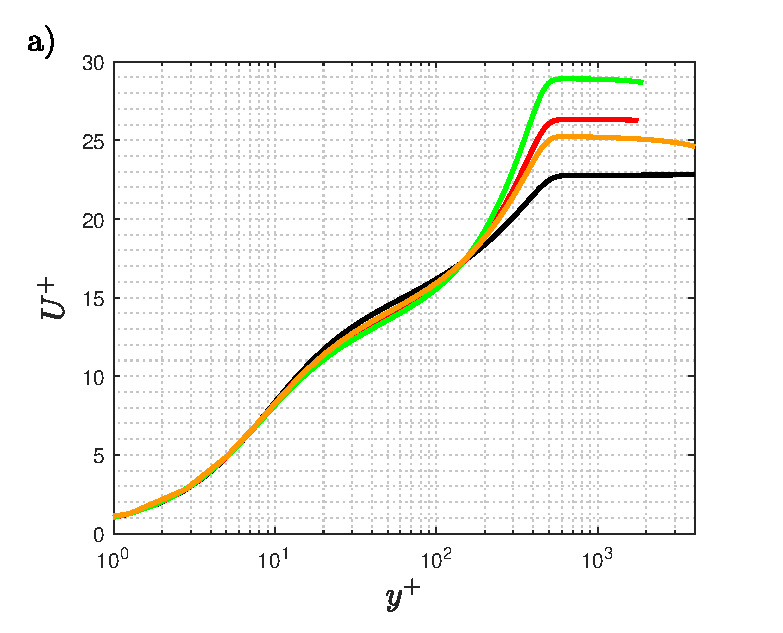
\includegraphics[width=0.49\textwidth]{fig21a.eps}
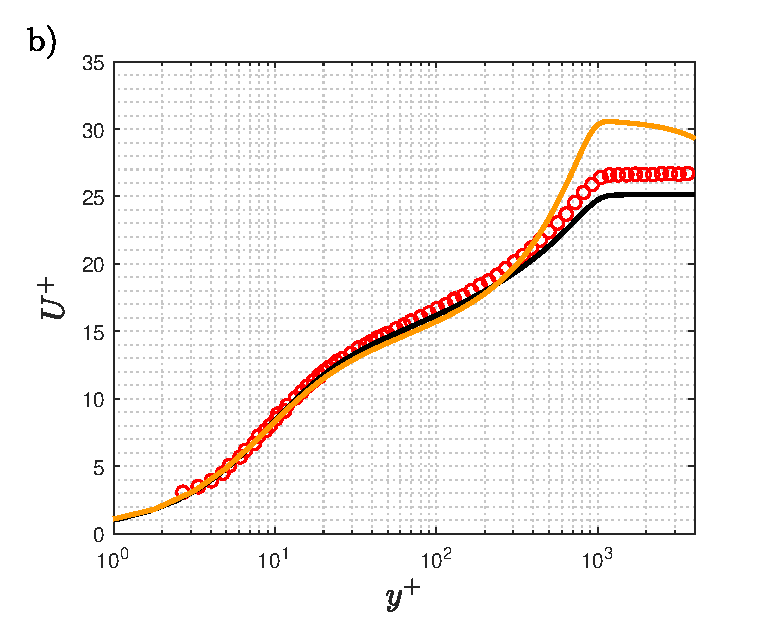
\includegraphics[width=0.49\textwidth]{fig21b.eps}
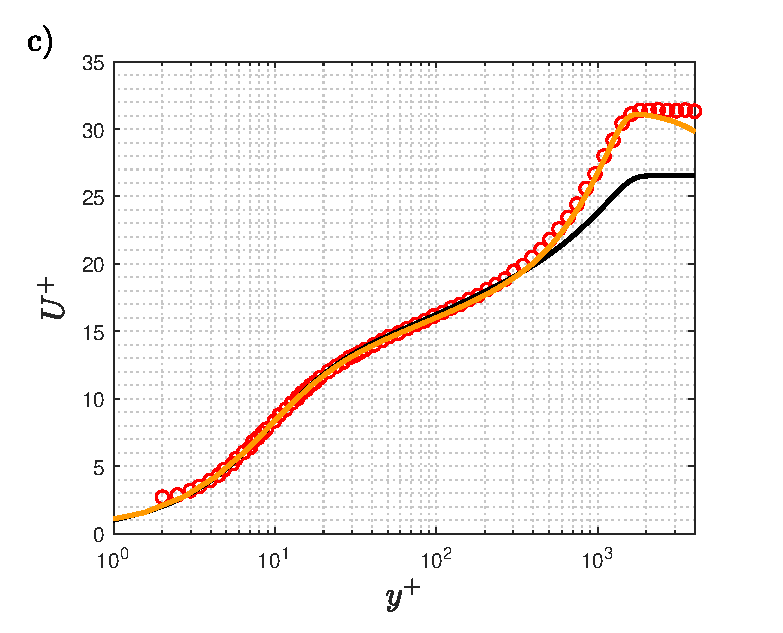
\includegraphics[width=0.49\textwidth]{fig21c.eps}
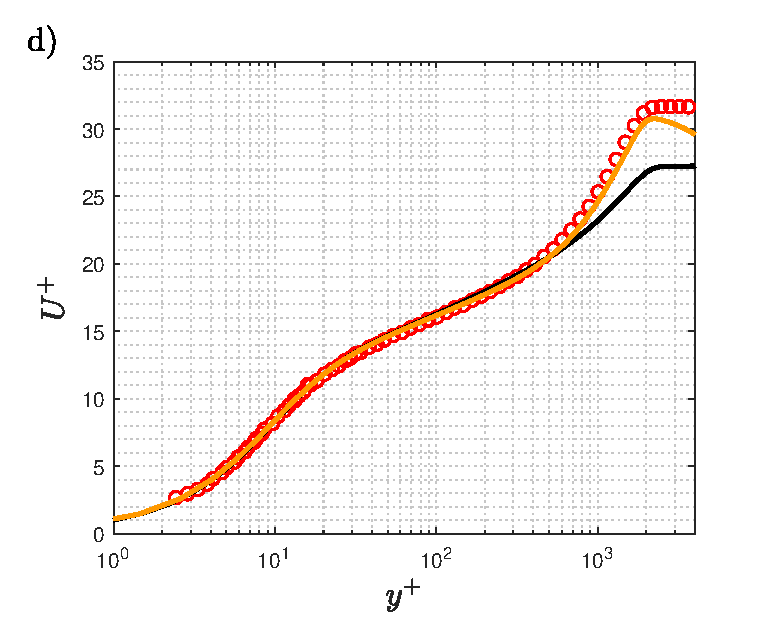
\includegraphics[width=0.49\textwidth]{fig21d.eps}
  \caption{ Inner-scaled streamwise mean velocity at different friction Reynolds numbers: a) $Re_{\tau}=500$ where $\beta(Re_{\tau})$ intersects for the simulations b1 and b1.4 ; b) $Re_{\tau}=1004$ ; c) $Re_{\tau}=1586$ ; d) $Re_{\tau}=2049$. Colors and symbols: (\protect\blackline) ZPG; (\protect\redline) b1; (\protect\orangeline) b1.4; (\protect\greenline) b2; (\protect\redcircle) exp; as in table \ref{tab:param}. }
\label{fig:meanU}
\end{figure}
 The mean streamwise velocity $U$ is represented in viscous scaling in figure \ref{fig:meanU}. It is possible to see the collapse for all the simulations for $y^+ \leq 10$. For the lowest $\Rey_{\tau}=500$, there is a difference in the buffer and logarithmic region, where an increasing APG is reflected in a lower $U^+$. Although b1 and b1.4 have the same $\beta \simeq 1.2$ at this $\Rey_{\tau}$, the b1.4 case has been exposed to lower values of $\beta$ in the upstream region than the b1 case. This is manifested in the buffer region, which exhibits a lower accumulated PG effect with its values being closer to the ZPG than those of the b1 APG. If we compared both curves at $\Rey_{\tau}=587$ where $c_f$ is the same for b1 and b1.4, we would be matching $U_e^+$ and both curves would show a better collapse; note that at this position the PG of b1.4 is higher and in the buffer region we could see that b1 is closer to the ZPG. This is also an example that even matching local $\Rey_{\tau}$ and $\beta$ does not imply a collapse of profiles as in \cite{tanarro_2020}, and the effects of the flow history need to be taken into account, not only the local states. At around $y^+=200$ the overlap region ends at these Reynolds numbers, and the curves diverge in the wake region, showing different values of $U_e^+$ since the $c_f$ are different.
Increasing the Reynolds number we can see a better collapse of the b1.4 and ZPG simulations along the inner region including the overlap layer. The APG effects are then confined to the wake region for the mean streamwise velocity. 


% Reynolds stress in outer units
\begin{figure}
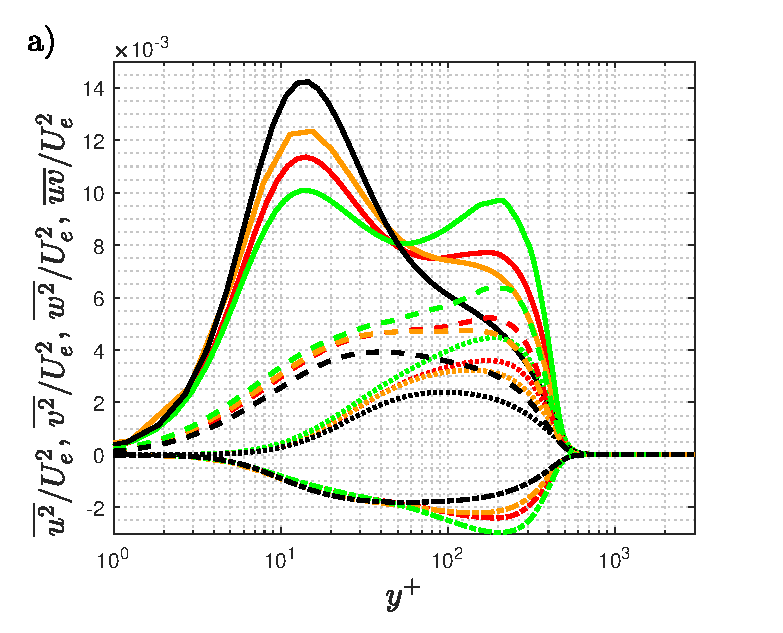
\includegraphics[width=0.49\textwidth]{fig22a.eps}
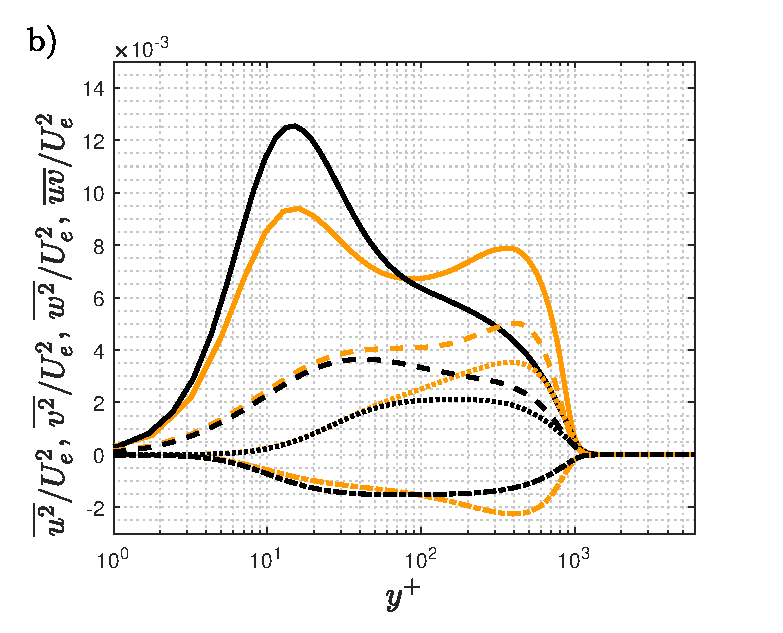
\includegraphics[width=0.49\textwidth]{fig22b.eps}
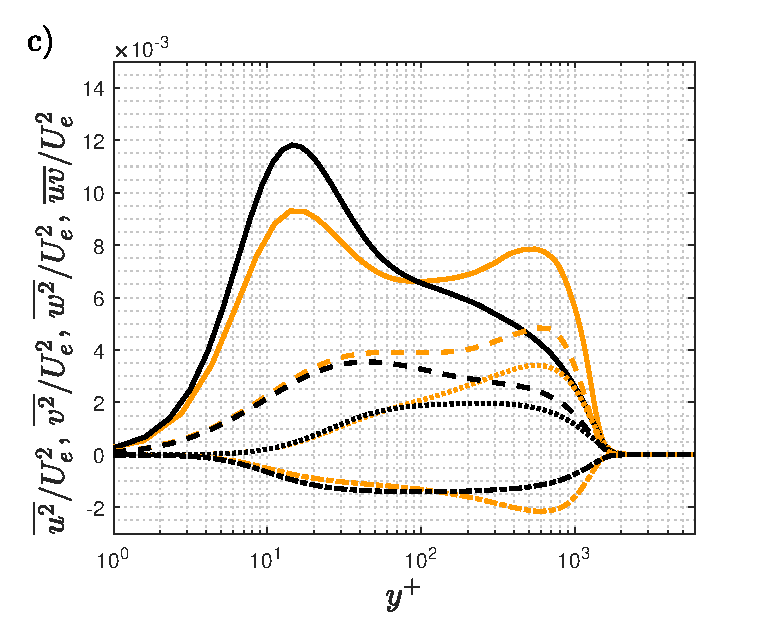
\includegraphics[width=0.49\textwidth]{fig22c.eps}
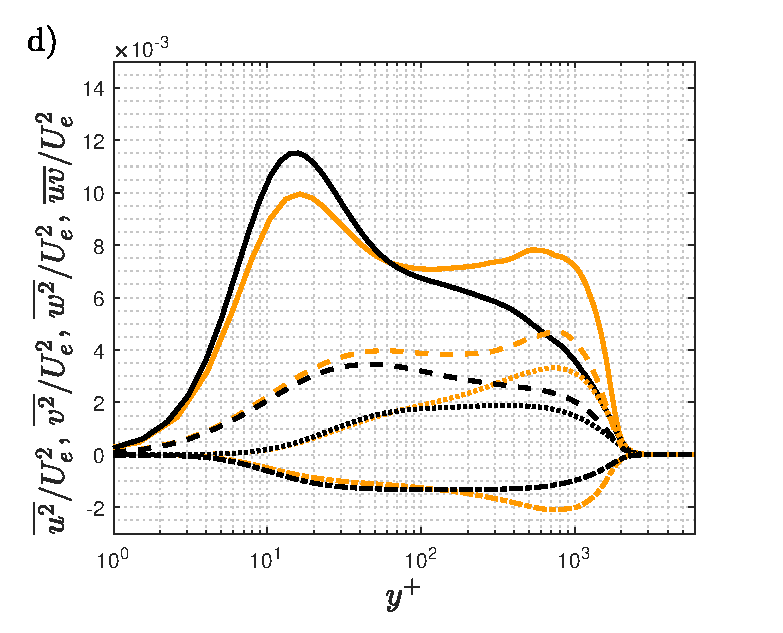
\includegraphics[width=0.49\textwidth]{fig22d.eps}
  \caption{ Reynolds stresses scaled with the edge velocity $U_e$ at various matched $Re_{\tau}$: a) $Re_{\tau}=500$ where $\beta(Re_{\tau})$ intersects for the simulations b1 and b1.4; b) $Re_{\tau}=1000$ ; c) $Re_{\tau}=1500$ ; d) $Re_{\tau}=2000$. Symbols: (\protect\blackline) $\overline{u^2}/U_e^2$; (\protect\blackdotted) $\overline{v^2}/U_e^2$; (\protect\blackdash) $\overline{w^2}/U_e^2$; (\protect\blackdashdot) $\overline{uv}/U_e^2$.  Colors as in table \ref{tab:param}. Colors and symbols: (\protect\blackline) ZPG; (\protect\redline) b1; (\protect\orangeline) b1.4; (\protect\greenline) b2; (\protect\redcircle) exp; as in table \ref{tab:param}. }
\label{fig:RSouter}
\end{figure}

\subsection*{  TKE-budget equations}
% ----------------------------------  TKE --------------------------
The transport equation of the TKE, defined as $\overline{k}=1/2( \overline{u^2} + \overline{v^2} + \overline{w^2} ) $, is decomposed into the following terms:

\begin{equation*}
     \frac{\partial }{\partial t} \overline{k} = P^k + \varepsilon^k + D^k + T^k  + \Pi^k + C^k ,
\label{eq:tke_bud}
\end{equation*}
 where the production term is computed as $P^k= - \overline{u_i u_j}({\partial U_i}/{\partial x_j})$, the dissipation as $\varepsilon^{k} = -\nu \overline{ ({\partial u_i}/{\partial x_j})^2}$ or $-2\nu (\overline{s_{ij}s_{ij}})$, (where $s_{ij}$ is the fluctuating strain rate), the viscous diffusion is defined as $D^k=(\nu/2)({\partial^2 \overline{u_iu_i}}/{\partial x^2_j})$, the velocity-pressure-gradient correlation $\Pi^k = -(1/\rho) ({\partial \overline{pu_i}}/{\partial x_i})$, the turbulent transport $T^k=-(1/2){\partial \overline{u_iu_iu_j}}/{\partial x_j})$ and the convection is $C^k=-(1/2)U_j({\partial \overline{u_iu_i}}/{\partial x_j})$. 


% TKE budget in inner units
\begin{figure}
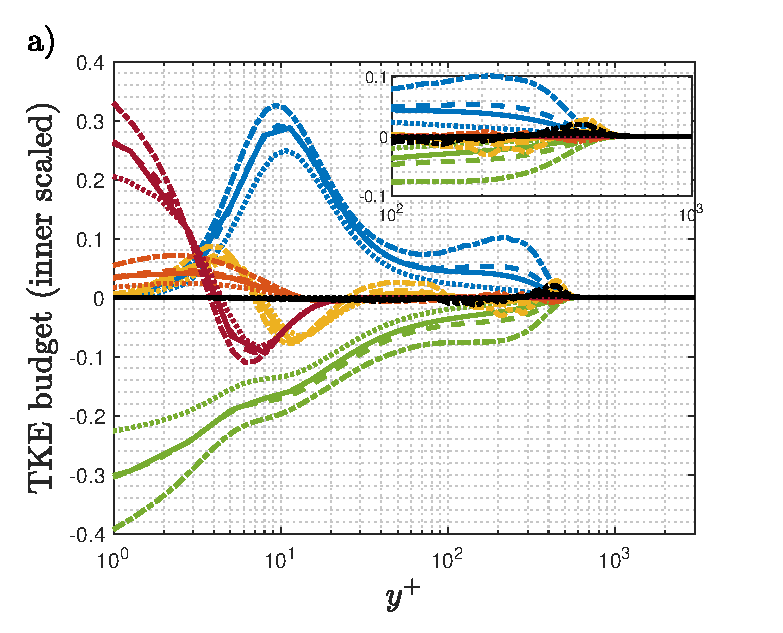
\includegraphics[width=0.49\textwidth]{fig23a.eps}
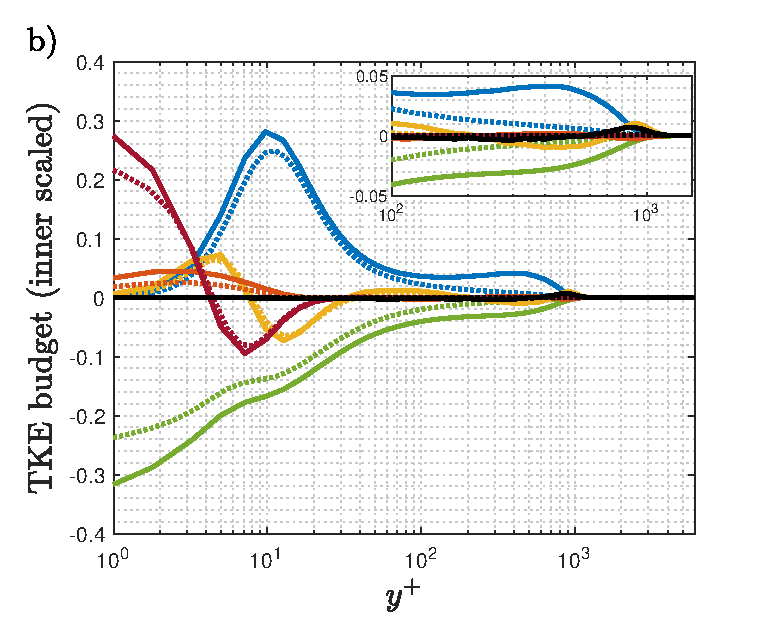
\includegraphics[width=0.49\textwidth]{fig23b.eps}
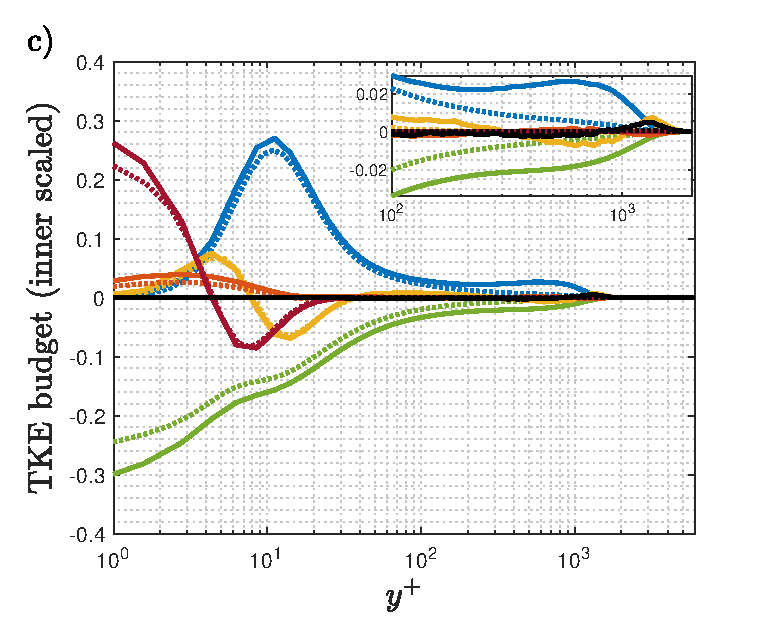
\includegraphics[width=0.49\textwidth]{fig23c.eps}
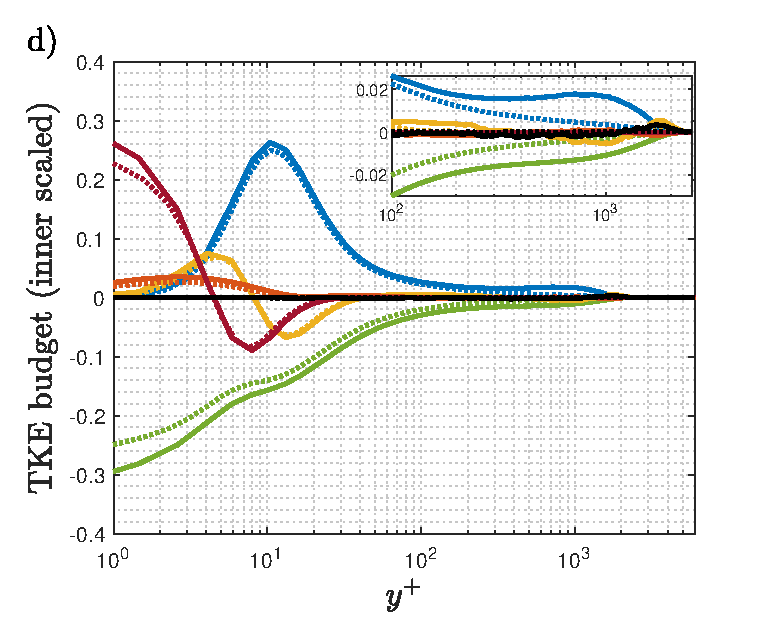
\includegraphics[width=0.49\textwidth]{fig23d.eps}
  \caption{ Inner-scaled turbulent-kinetic-energy budget at different $Re_{\tau}$: (Top-left) $Re_{\tau}=500$ where $\beta(Re_{\tau})$ intersects for the simulations b1 and b1.4 . (Top-right) $Re_{\tau}=1000$, (bottom-left) $Re_{\tau}=1500$, (bottom-right) $Re_{\tau}=2000$. Symbols: (\protect\blackline) b1.4; (\protect\blackdotted) ZPG; (\protect\blackdash) b1 and (\protect\blackdashdot) b2. The colours correspond to the following terms of the TKE budget: production (\protect\blueline), dissipation (\protect\greenline), turbulent transport (\protect\yellowline), velocity-pressure-gradient correlation (\protect\orangeline), viscous diffusion (\protect\magentaline) and convection (\protect\blackline).}
\label{fig:TKEinner}
\end{figure}


% TKE budget in outer units
\begin{figure}
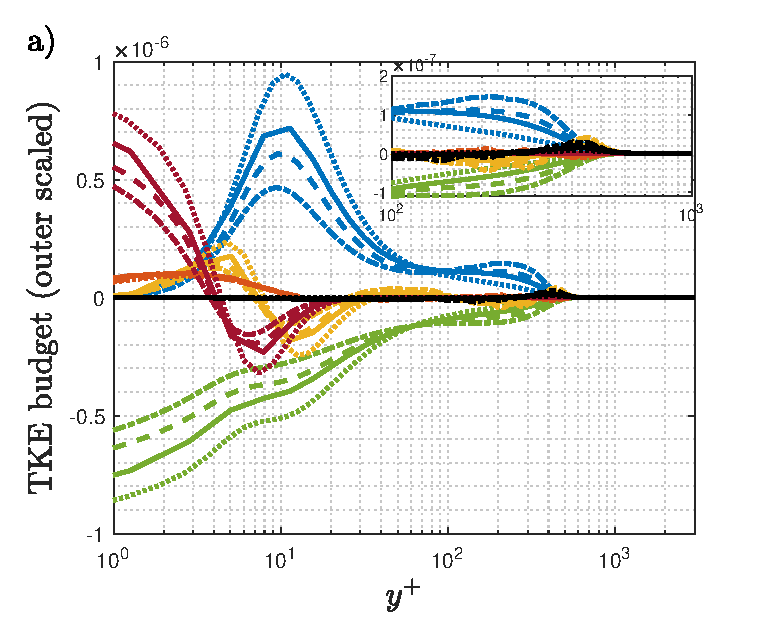
\includegraphics[width=0.49\textwidth]{fig24a.eps}
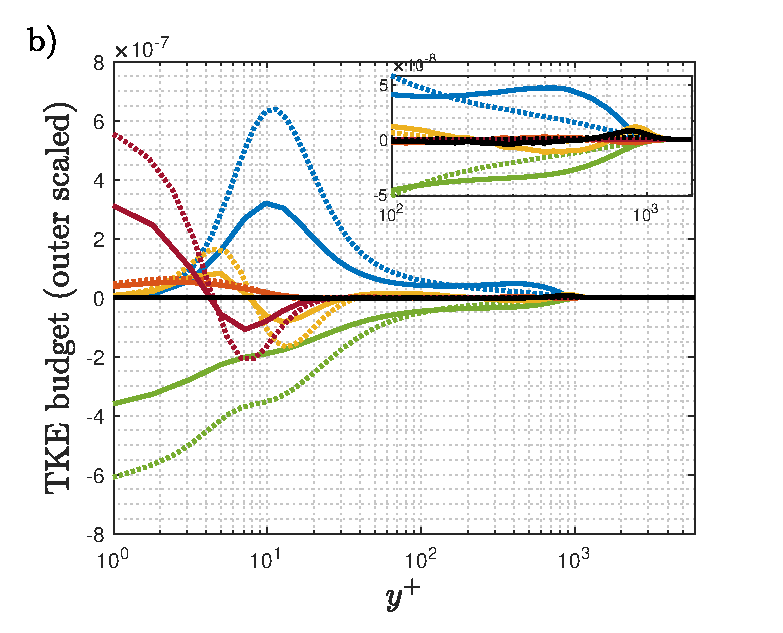
\includegraphics[width=0.49\textwidth]{fig24b.eps}
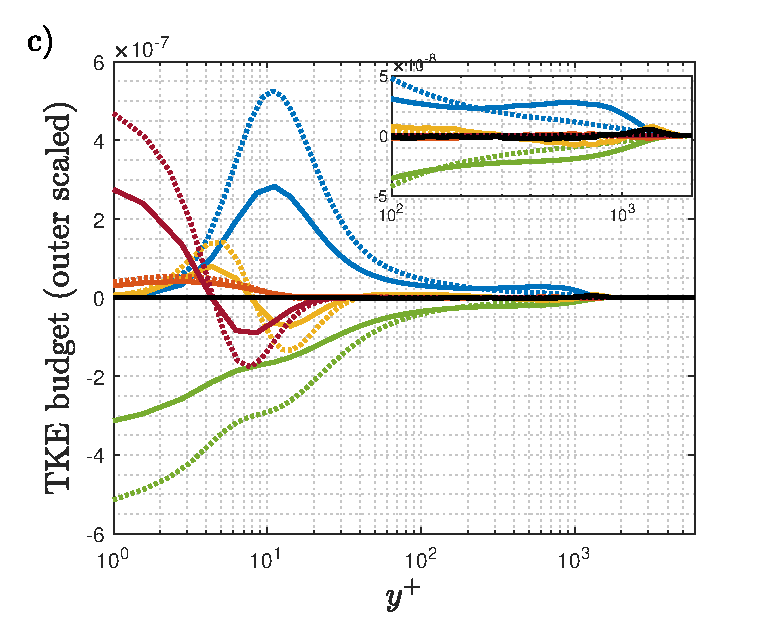
\includegraphics[width=0.49\textwidth]{fig24c.eps}
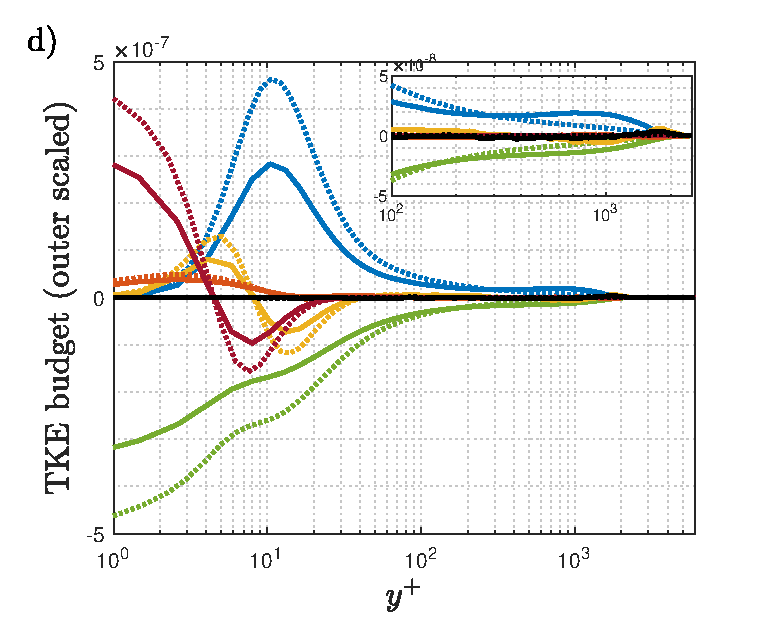
\includegraphics[width=0.49\textwidth]{fig24d.eps}
  \caption{ Outer-scaled turbulent-kinetic-energy budget at different $Re_{\tau}$: (Top-left) $Re_{\tau}=500$ where $\beta(Re_{\tau})$ intersects for the simulations b1 and b1.4 . (Top-right) $Re_{\tau}=1000$, (bottom-left) $Re_{\tau}=1500$, (bottom-right) $Re_{\tau}=2000$. Symbols: (\protect\blackline) b1.4; (\protect\blackdotted) ZPG; (\protect\blackdash) b1 and (\protect\blackdashdot) b2. The colours correspond to the following terms of the TKE budget: production (\protect\blueline), dissipation (\protect\greenline), turbulent transport (\protect\yellowline), velocity-pressure-gradient correlation (\protect\orangeline), viscous diffusion (\protect\magentaline) and convection (\protect\blackline).}
\label{fig:TKEouter}
\end{figure}

 
The turbulent-kinetic-energy (TKE) budgets are shown in inner scale in figure~\ref{fig:TKEinner} and in outer scale in figure~\ref{fig:TKEouter}. As seen before in the inner region of the streamwise RS, the magnitude of the various budget terms increases in inner scaling with the APG, as opposed to the behaviour in outer scale where the APG produces a reduction of these magnitudes. 

Figure \ref{fig:TKEinner} shows that, as the distance from the wall is increased, differences in the velocity-pressure-gradient correlation are observed.

As the Reynolds number is increased, the general magnitude of each TKE-budget term as well as the relative differences between the various simulations are reduced. The most prominent effects of the APG are seen in the viscous sub-layer for the pair viscous-diffusion/dissipation and in the wake region for production/dissipation.
The outer scaling leads to an excellent collapse of the velocity-pressure-gradient correlation for all the simulations in all the regions of the TBL.
The phenomena discussed above for the Reynolds-stress terms where the APG leads to the development of an outer peak in all the components of the tensor, is manifested here as a second peak in the TKE production and dissipation in the outer region. Note that while the near-wall production peak becomes progressively smaller for higher $\beta$ when scaled in outer units, the outer-production peak exhibits the opposite behavior and grows with $\beta$. The value of $\beta$ decreases slowly in b1.4 with Reynolds number, and the outer peak in the TKE budget terms is also reduced at higher $\Rey$, approaching the ZPG values in inner scale.


   
The equations for the different terms of the TKE budgets are the same for ZPG and APG, but the magnitude of the streamwise gradients ($\partial / \partial x$) is larger in the APG compared to the ZPG.
We will analyze the major differences seen for the production $P^k=-\overline{u^2}\partial U/ \partial x -\overline{v^2}\partial V/ \partial y -\overline{uv} (\partial U/ \partial y + \partial V/ \partial x)$ in inner units.
   
The largest contribution to $P^k$ is given by the third term $-\overline{uv} \partial U/ \partial y$, which is much larger than the other three. 

   
In the inner region the main differences come from the first two terms, since the magnitude of $\partial U/ \partial x$ for APGs is greater than for the ZPG and as a result of the continuity equation, the magnitude of $\partial V/ \partial y$ is also larger for APG than for ZPG. As discussed above, a larger $\beta$ leads to a larger inner-scaled near-wall peak of $\overline{u^2}$ for the APG than for the ZPG, therefore the first term of $P^k$ is also larger. In the outer region of the APG, all the terms in the RS tensor exhibit an outer peak, and these outer peaks, together with the gradients of $U$ and $V$ being larger than in the ZPG, produce an outer peak in the production term. Note from figure \ref{fig:meanU} that the slope of $U$, which is $\partial U/ \partial y$, is larger for APG than for the ZPG.



